\chapter{Company presentation}

\section{Field of activity}
\subsection{Wind energy}
Upteko has been manually inspecting wind-turbines since 2018. Today, they are using this data and knowledge to build a system to automatically inspect wind turbines
Upteko's autonomous drone system will provide high-quality aerial data for all inspections and maintenance requirements, in a safer, more efficient manner, without causing operational downtime.
Their drones are pre-programmed with geo-referenced 3D trajectories for the inspection of wind turbines. While flying the planned routes, several images are acquired. The actual number depends on the camera specification, flight altitude and post-processing performance (overlap between images). All images are georeferenced using the UAV position at the acquisition time and these images are afterwards stitched together and in one picture on which the locations of the damages are shown.
They deliver these data as per the clients' requirements in raw files or provide a damage report that explains the severity of damages from type 1 to type 5.

\subsection{Oil and Gas}
Upteko is working on a solution for detecting oil spills on the surface of the water. They are developing payloads for their drone system that can help detect the signature of oil floating on water surfaces. This payload can be installed on Lärke and can be used to automatically or manually detect oil spills.
Upteko have developed an application to detect pirate attacks on off-shore oil rigs and large commercial ships. Pirates use small ships to attack these oil rigs and large commercial ships at night. They take the crew and contents hostage. There are no mobile long-range detection tools with aerial insight to give the crew information about nearby pirates. This results not only in huge loss to the oil industry but also endangers the crew at huge life risks.
The total cost of piracy to the shipping industry, from insurance and time lost, is estimated at over €6B/year.
Upteko's multipurpose drone system has a feature called perimeter control. This feature allows any member of the crew to investigate surrounding vessels approaching the premises. A built-in feature within the drone system is added to allow a crew member to operate and control the aerial camera in any direction with no prior drone experience. The geothermic cameras and the infrared sensors help to detect the approach of any pirates faster even during night-time.

\subsection{Offshore and Maritime}
Upteko has been consistently involved with the maritime industry since its inception. They are developing a drone system solution to live on the ship, to connect port operations on the ground and at the sea, with insight from the sky. This system includes a drone and a charging station for the drone that will be installed on the ship. The drone can autonomously perform a variety of tasks and then fly back and charge its batteries while staying protected against the weather. 
With an in-depth understanding of the challenges that the maritime industries face in attempting long and expensive inspections and other operational tasks, Upteko's software and hardware drone system allows a 100\% automatic inspection of a ship in less than 2 hours. 
Having a permanent drone on a ship will be extremely helpful in a number of cases that can range from Search and Rescue (SAR) operations, vessel docking, dry dock inspections, fire hazard detection and situational awareness among other functionalities.

\section{History}
Upteko™ was founded in 2018 by Mads Joergensen, Benjamin Mejnertz, and Sebastian Duus to pursue the opportunity of developing drone applications for the maritime sector. For Benjamin and Sebastian, it started as a hobby, competing in RC Helicopter competitions around the world and later became a business worth pursuing. Mads came onboard, and together they created Upteko and built a great team of experienced drone pilots, software- and hardware engineers, and business developers. Today Upteko has offices located in Copenhagen, Odense, and Skanderborg. Upteko is about using their creativity and initiative to become leaders in the drone industry.
To develop fitting solutions to your needs, they value collaboration and co-creation highly among external parties. Through several years of collaborating with their customers, complementary assets providers, and even competitors, they have achieved priceless partnership within the maritime and other sectors. They are continuously on the hunt for new collaborations.

\section{Legal and social model}
In Denmark, most companies operate under a legal structure of a private limited company (Anpartsselskab, ApS) as Upteko. The country has strong social welfare systems and labor laws, which mandate fair treatment and protection of employees. Danish companies usually have a strong focus on maintaining a healthy work-life balance and uphold high ethical standards, both socially and environmentally.

\section{Economic model}
Denmark follows a mixed-market capitalist system, combining free market principles with a strong regulatory oversight. Upteko operates under a model of sustainable growth, focusing on long-term stability rather than short-term profits. This includes social responsibility, ethical business practices, and environmental sustainability.

\section{Type of work organization}
Denmark has a distinctive workplace culture, often characterized by a flat organizational structure. This implies low power distance, high levels of trust, and extensive collaboration between different levels of the organization. Danish companies typically have strong communication and decision-making practices, promoting employee empowerment and autonomy.
Upteko is organised in three main sectors : \texttt{Technical Development}, \texttt{Finance} and \texttt{Product management}. Here is the actual organization chart of the company :
\begin{center}
    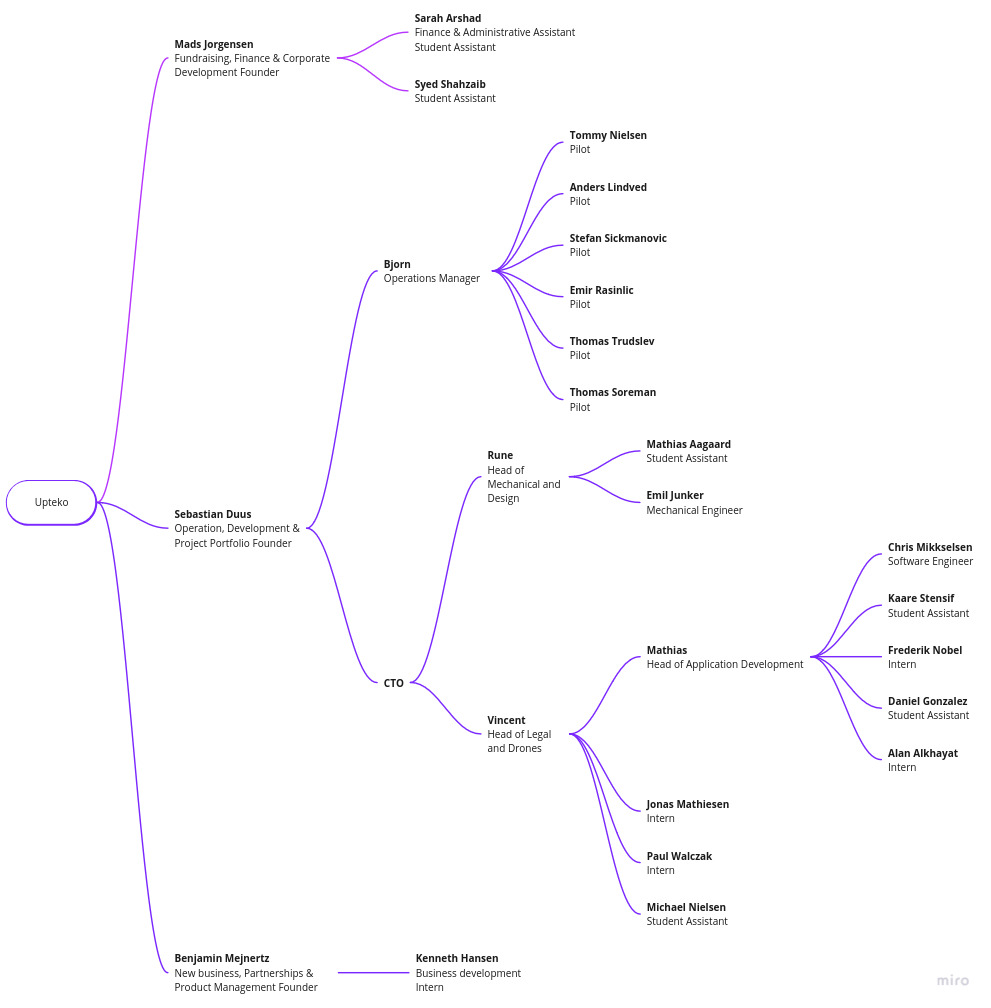
\includegraphics[width=1.0\linewidth]{./company_presentation/upteko_organization.jpg}
\end{center}